\chapter{Architecture}
In the MoVEAS' previous version, developed and improved by Dario Piotrowicz \cite{Pio19} and Yvonne Vulcano \cite{Vul19} from the Marco Lanini's project \cite{Lan17}, can be split into two major components: the client-side part, to collect, filter and send to the server the sensors' data, and the server-side one, to receive and manage that data.
\bigbreak

The Particle Photons, the sensors and the batteries are installed inside two toys: and airplane and a cement mixer truck.

\section{Client-side}
The data collected from the Photon basically flowed like as shown in the following schema:

\begin{center}
	\begin{figure}[ht!]
		\makebox[\textwidth]{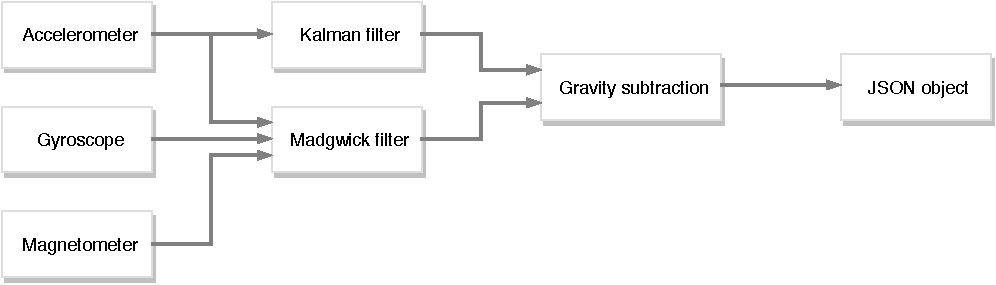
\includegraphics[width=0.65\paperwidth]{img/data_fusion_old.pdf}}
		\caption{Previous project's data fusion schema.} \label{old data fusion schema}
	\end{figure}
\end{center}
\bigbreak

As shown in the chapter \ref{Madgwick filter}, the Madgwick filter does not need Kalman-filtered data: that's why it takes the raw sensors' output. Then the Kalman-filtered acceleration is used jointly to the heading estimation given by the Madgwick filter, to subtract the gravity's acceleration – although there are some few residues, about 0.05g.
\bigbreak

There are 2 threads that are run in parallel in the devices:
\begin{itemize}
	\item one that constantly reads data from the sensors and updates the filters, as fast as it can;
	\item one that is woken up at the frequency of 22Hz, reads the data from the filters and from the program variables, packs up them into a JSON object, and sends it to the server.
\end{itemize}

\section{Server-side}
The Node.js server is basically composed by two modules:
\begin{itemize}
	\item the \textit{play session} module, that allows to record a session related to a specific patient, manage the recorded sessions, and visualize the saved ones with the moving 3D model (eventually along with the video recording) and the neural network classification of the movement;
	\item the \textit{pattern recording} module, that allows to record new training examples for making up the neural network's training and testing set, and to manage the pattern's labels and all the samples related to them.
\end{itemize}
In both cases the data sent by the device is used for the real-time 3D representation of the toy's model.
